\chapter{Experiments and Results}
\label{experiments}

This chapter introduces in greater detail the data and results for the thesis project. We perform three experiments. The first is an analytic experiment, constructed as a proof of concept to confirm the basic premise that the \cvae{} can be used to predict conditional distributions. In the following experiments we evaluate the \dettostoc{} algorithm in two different scenarios using a physics engine.

Some questions we want to answer: How does \dettostoc{} compare against a baseline model? How many iterations of \dettostoc{} are required for \fdecoder{} to match \fsimulator{} with sufficient accuracy?

\section{Evaluation}
Evaluating the performance of a generative model is not straightforward. We therefore choose to present the results in several ways. The generative model learns a multivariate normal distribution with means $\vec{\mu}$ and a diagonal covariance matrix $\vec{\Sigma} = \vec{\sigma^2}\times\vec{I}$. The most important metric is the log likelihood of the test set $\trajrealtest$

\begin{equation}
    \log \mathcal{L} = -\frac{N}{2} \log \vert \vec{\Sigma} \vert - 
    \frac{1}{2} \sum^N_{i=1} (\vx_i - \vec{\mu})^T \vec{\Sigma} (\vx_i - \vec{\mu}) 
\end{equation}

This yields a number indicating the goodness of fit, but a scalar is not very helpful in order to understand the quality of the predictions without comparison. We consequently contrast it with a baseline model. We also visually display results whenever possible to further demonstrate how the models perform.

\subsection{Baseline model}
We compare the results of \dettostoc{} against a \emph{baseline} \cvae{} with the same number of layers and hidden units. Given infinite data, the baseline model should provide good generative results. The baseline \cvae{} is trained strictly on \emph{real} data which is limited, and serves as an indication of the predictive performance without alignment with simulation data.

\section{Analytic experiment}
\label{exp:analytic}
As an initial experiment we use data with known distributions that can easily be analyzed. We define a joint distribution $p(s,s',\psi)$ and then attempt to learn the conditional distribution $p\given{s'}{s,\psi}$. If the distribution is a multivariate Gaussian, then the conditional distribution is also Gaussian and we can find analytic expressions for its mean and covariance \parencite{bishop:2006:PRML}. In the general case, if $\vx$ is a multivariate Gaussian variable of dimension $l+m$, we can partition $\vec{Z}$ into two multivariate variables $\vx_a$ and $\vx_b$

\begin{equation}
\vec{\vx} = 
\begin{bmatrix}
\vec{\vx_a} \\
\vec{\vx_b}
\end{bmatrix}
\quad
\text{with sizes:} 
\begin{bmatrix}
l \\
m
\end{bmatrix}
\end{equation}
We find the mean and covariance by
\begin{equation}
\mu_{\vx} = 
\begin{bmatrix}
\vec{\mu}_{a} \\
\vec{\mu}_{b}
\end{bmatrix}
\quad
\text{with sizes:} 
\begin{bmatrix}
l \\
m
\end{bmatrix}
\end{equation}

\begin{equation}
\vec{\Sigma}_{\vx} = 
\begin{bmatrix}
\vec{\Sigma}_{aa} & \vec{\Sigma}_{ab} \\
\vec{\Sigma}_{ba} & \vec{\Sigma}_{bb}
\end{bmatrix}
\quad
\text{with sizes:} 
\begin{bmatrix}
l\times l & l \times m\\
m \times l & m \times m
\end{bmatrix}
\end{equation}
\\
The conditional distribution $p\given{\vx_a}{\vx_b}$ can then be identifying by completing the square resulting in
\begin{align}
%\E[X \vert Y = y]
\vec{\mu}_{\given{a}{b}} &= \vec{\mu}_{a} + \vec{\Sigma}_{ab}\vec{\Sigma}_{bb}^{-1}(\vec{x}_b - \vec{\mu}_{a})
\label{eq_cond_mean}
\\
%Cov[X \vert Y = y]
\vec{\Sigma}_{\given{a}{b}} &= \vec{\Sigma}_{aa} - \vec{\Sigma}_{ab}\vec{\Sigma}_{bb}^{-1}\vec{\Sigma}_{ba}
\label{eq_cond_var}
\end{align}

The question is now is to see if it is possible to learn $\vec{\mu}_{\given*{a}{b}}$ and $\vec{\Sigma}_{\given{a}{b}}$ using a \cvae{}.

% \begin{figure}
% \begin{center}
% 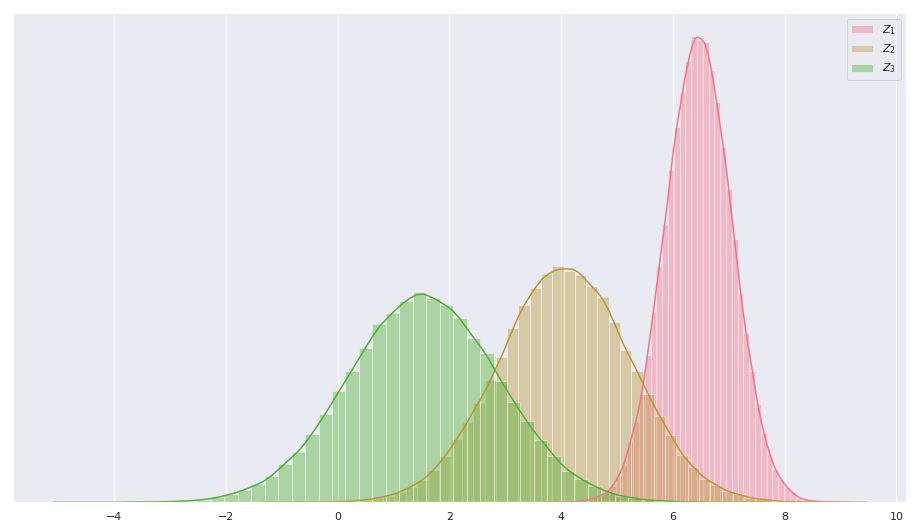
\includegraphics[width=0.8\textwidth]{img/trivariate}
% \caption{Example showing density for each univariate distribution given samples from a trivariate distribution $p(s, a, s')$.}
% \end{center}
% \end{figure}

%\subsection{Training procedure}

To setup this experiment, we randomly generate the parameters of a trivariate Gaussian distribution and ensure the covariance matrix is positive semi-definite. The \cvae{} is trained with samples from the trivariate distribution in the following way:

First, we sample $(s, a, s')$ from the trivariate distribution. Then, the probabilistic encoder is used to produce $\qphi \given{z}{s', s, a}$. We then modulate the posterior $z$ with the conditional inputs $s, a$ and use the decoder to predict the distribution $\ptheta \given{s'}{z, s, a}$. We can view this as analogous to the goal of learning the next state $s'$ conditioned on the current state $s$ and control actions $a$.

\begin{figure}
\centering
\captionsetup{size=footnotesize}
\begin{subfigure}{\linewidth}
  \centering
  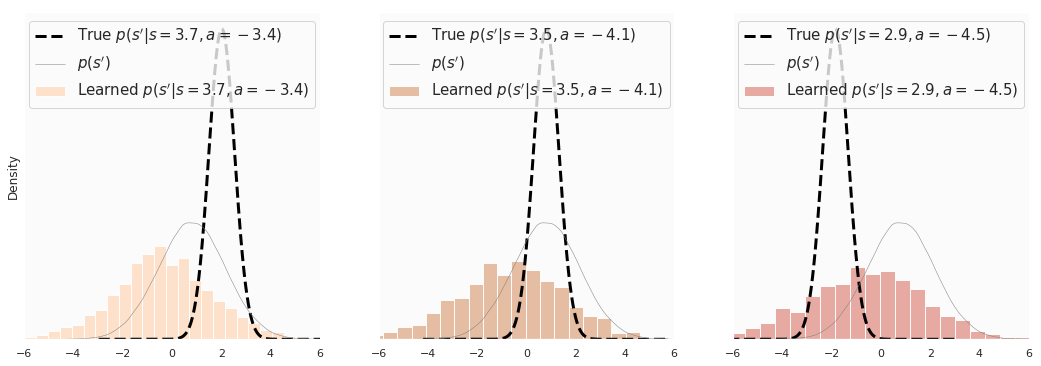
\includegraphics[width=0.9\linewidth]{img/trivariate/trivariate_step0}
  \caption{0 gradient steps}
\end{subfigure}
\begin{subfigure}{\textwidth}
  \centering
  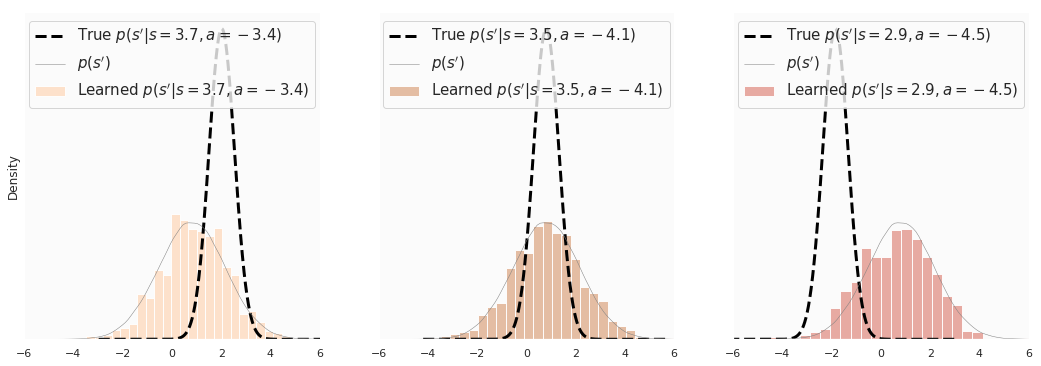
\includegraphics[width=0.9\linewidth]{img/trivariate/trivariate_step100}
  \caption{100 gradient steps}
\end{subfigure}
\begin{subfigure}{\textwidth}
  \centering
  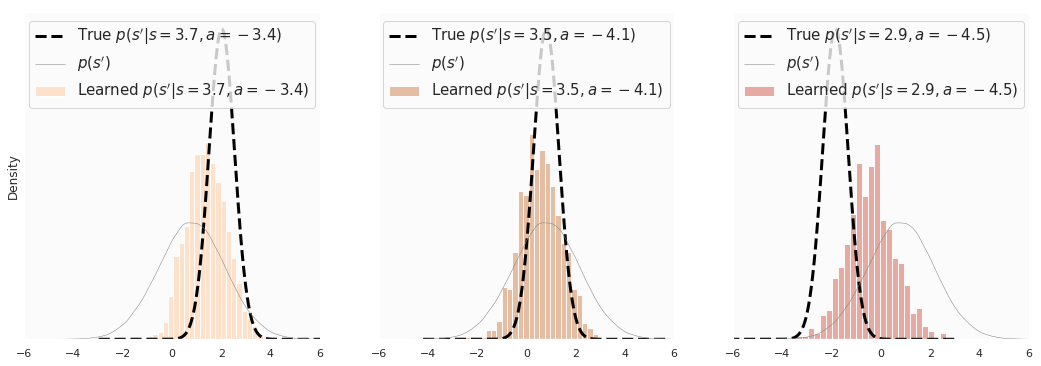
\includegraphics[width=0.9\linewidth]{img/trivariate/trivariate_step500}
  \caption{500 gradient steps}
\end{subfigure}
\begin{subfigure}{\textwidth}
  \centering
  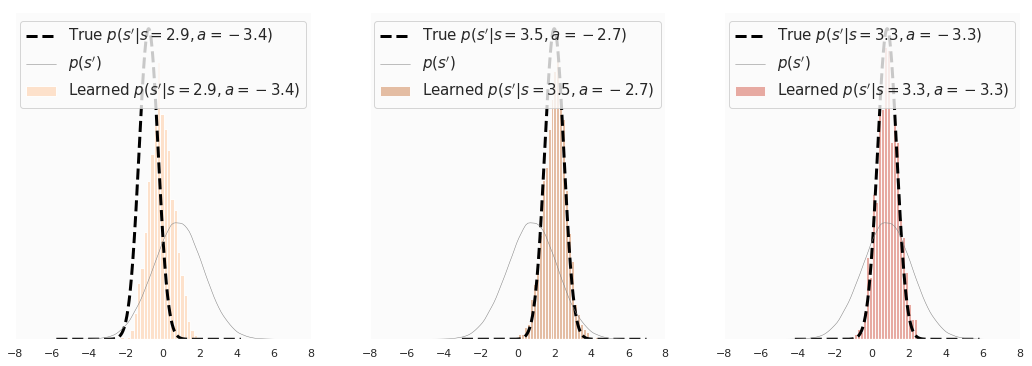
\includegraphics[width=0.9\linewidth]{img/trivariate/trivariate_step2000}
  \caption{2000 gradient steps}
\end{subfigure}

\caption[]{Three different density estimations during training for \ensuremath{p \given*{s'}{a,s}} where $a$ and $s$ have been randomly sampled from a known trivariate distribution in each plot and drawn as vertical lines. The expected density $p \given{s'}{s, a} \sim \N (\mu_{\given{s'}{s,a}}, \Sigma_{\given{s'}{s,a}})$ is computed using equations \ref{eq_cond_mean} and \ref{eq_cond_var} and its outline plotted in thick dashed lines.}
\label{fig:trivariate_density}
\end{figure}

As illustrated by Figure \ref{fig:trivariate_density}, the \cvae{} initially learns the distribution $p(s')$ but ultimately converges towards the true computed conditional distribution $p \given{s'}{s, a} \sim \N (\mu_{\given{s'}{s,a}}, \Sigma_{\given{s'}{s,a}})$ after training on enough samples. %That is, the \cvae{} begins learning by ignoring the condition $s, a$, and instead memorizes the distribution $p(s')$, but after seeing enough samples it eventually learns to consider the condition and accurately predicts the conditional distribution $p \given{s'}{s, a}$.

\section{The MuJoCo simulator and scenarios}

MuJoCo \parencite{todorov2012mujoco}, short for Multi-Joint dynamics with Contact, is a physics engine, suited in particular for simulating complex dynamic systems in contact-rich scenarios. Performance on robotics-like scenarios simulated by MuJoCo is frequently reported when analyzing performance of RL algorithms~\parencite{duan2016benchmarking, popov2017data}.

For these experiments, we construct scenarios in MuJoCo and select parameters $\vec{\psi}$ that we wish to learn to reduce the reality gap. %We then observe the scenarios with a distribution over these parameters $\vec{\psi}$. 

In this context and the following two experiments, \textit{real} data refers to trajectories generated via the simulator with a configuration of the parameters with slight Gaussian noise. The choice of means are picked at random, and the variances are selected to be small yet slightly stochastic to resemble the unpredictability of the real world. This noise is introduced during simulation and not added to observations. While this does not guarantee that \dettostoc{} works on actual real-world data, there are other benefits to conducting the experiments this way. One positive bonus with synthesizing \emph{real} data is that we can generate a variety of different physics dynamics to represent alternative versions of ''reality'' and make sure that the algorithm can find the correct set of parameters that best represent that particular system. Moreover, a plethora of test data can be generated to verify the quality of the results.

\subsection{Parameters and their meanings}
In the following experiments when we refer to friction we mean isotropic tangential friction between two geoms in MuJoCo. In MuJoCo, wind is a vector that is subtracted from the 3D translational velocity of each body, and the result is used to compute viscous, lift and drag forces acting on the body in passive dynamics. In the Windy Slope scenario, wind is only used along one axis, perpendicular to the inclination of the slope and thus causes the box to move sideways. Table \ref{table:mujoco_parameters} defines the notation we use for the following experiments with the corresponding MuJoCo API. For more information about how MuJoCo computes friction, contact detection and other forces, please see the Computation part at: \url{mujoco.org/book/computation.html}.

\begin{table}
\ra{1.3}
\centering

\begin{tabular}{lr}
\toprule
Notation & MuJoCo parameter \\
\midrule
$\pfriction{}$ & \texttt{mjModel.pair\_friction} \\
$\pcom$ & \texttt{mjModel.geom.pos} \\
$\pwind$ & \texttt{mjOption.wind} \\
\bottomrule
\end{tabular}
\caption{Variable notation and their respective parameter in the MuJoCo API.}
\label{table:mujoco_parameters}
\end{table}


\section{Windy Slope scenario}
\label{windyslope}

\begin{figure}
\begin{subfigure}{\textwidth}
  \centering
  \begin{overpic}[trim=800 100 800 300,clip,width=0.3\textwidth]{img/windyslope/traj/windyslope-real-0}
      \put(2,2) {\color{white}$t=0$}
  \end{overpic}
  \begin{overpic}[trim=800 100 800 300,clip,width=0.3\textwidth]{img/windyslope/traj/windyslope-real-all-obstacle-50}
      \put(2,2) {\color{white}$t=50$}
  \end{overpic}
  \begin{overpic}[trim=800 100 800 300,clip,width=0.3\textwidth]{img/windyslope/traj/windyslope-real-all-obstacle-100}
      \put(2,2) {\color{white}$t=100$}
  \end{overpic}
\end{subfigure}

\caption{The \ws{} scenario, where a box with hidden inner content is placed on a sloping surface exposed to wind. The figure shows the environment at different timesteps $t$, and the position and orientation of the box have been superimposed in each image to give a sense of the randomness over time. The trajectory depends on samples from the slightly noisy \textit{real} parameter distributions: $\pfriction \sim \N(0.23, 0.01^2)$, $\pcom \sim \N(0.11, 0.04^2)$ and $\pwind \sim \N(-1.7, 0.05^2)$.}
\label{fig:windyslope_real}
\end{figure}

A first scenario was constructed using MuJoCo in order to see if the \dettostoc{} algorithm can predict the next state given the current state while only simulating passive dynamics.

In this scenario, which can be seen in Figure \ref{fig:windyslope_real}, an object is placed on a sloping surface. To make the scenario more challenging and to emulate a situation where a parameter cannot be measured, another object is placed inside the box at an unknown position, as seen in Figure \ref{fig:inside_box}. Thus, the center of mass of the box is altered as the inner object slightly moves. Furthermore, a fixed cylindrical obstacle placed in the middle of the surface, since accurately modelling contact is difficult and should make predicting the output somewhat harder. 

\begin{figure}
\centering
    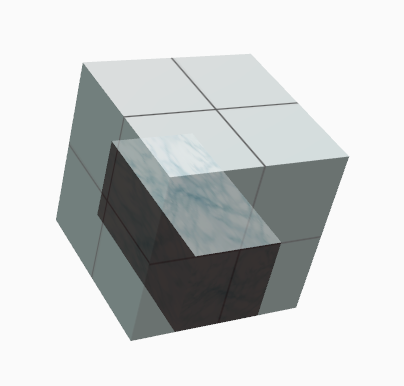
\includegraphics[trim=0 0 0 0,clip,width=0.3\textwidth]
    {img/windyslope/windyslope_inside}
    \caption{The object inside the box. The box has been made transparent to show the contents of the box: a brick whose position affects the center of mass of the box.}
    \label{fig:inside_box}
\end{figure}

How the box moves on the surface depends on the following variables: the tangential friction coefficients between the surface and the box, $\pfriction$, its center of mass, $\pcom$, as well as viscous, lift and drag forces caused by wind, $\pwind$. How these parameters each affect the environment is illustrated in Figure \ref{fig:windyslope_psi}. The goal is to predict the next state $\vns$ given current state $\vs$, with no knowledge of the \textit{real} variables for friction, wind and the position of the inner object. The state is an 18D vector consisting of the current position, orientation, linear and angular velocity of the object.

Following the \dettostoc{} algorithm outlined in \ref{det2stoc:algorithm}, we define initial distributions in parameter space $\vec{\psi}$ as wide truncated Gaussians. For this experiment, these initial estimates are purposely made uninformative as a proof of principle. For example, the prior distribution for $\pwind$ implies we do not know which way the wind is blowing. In reality however, the estimates can be based on observing the dynamics in the real world and trying to replicate the same behavior in the simulator.

\begin{figure}
\centering
\begin{subfigure}{0.85\linewidth}
\begin{subfigure}{\linewidth}
    \centering
    \begin{overpic}[trim=900 200 800 400,clip,width=0.4\linewidth]{img/windyslope/traj/windyslope-friction-50}
        \put(2,2) {\color{white}$t=50$}
    \end{overpic}
        \begin{overpic}[trim=900 200 800 400,clip,width=0.4\linewidth]{img/windyslope/traj/windyslope-friction-99}
        \put(2,2) {\color{white}$t=100$}
    \end{overpic}
    \caption{$\vec{\pfriction} \sim \N(0.25,0.1)$ with $\vec{\pwind}$ and $\vec{\pcom}$ fixed.}
    \label{fig:traj_friction}
\end{subfigure}
%
\begin{subfigure}{\linewidth}
    \medskip
    \centering
    \begin{overpic}[trim=900 200 800 400,clip,width=0.4\linewidth]{img/windyslope/traj/windyslope-fake-wind-50}
        \put(2,2) {\color{white}$t=50$}
    \end{overpic}
        \begin{overpic}[trim=900 200 800 400,clip,width=0.4\linewidth]{img/windyslope/traj/windyslope-fake-wind-99}
        \put(2,2) {\color{white}$t=100$}
    \end{overpic}
    \caption{$\vec{\pwind} \sim \N(-1.0,0.5)$ with $\vec{\pfriction}$ and $\vec{\pcom}$ fixed.}
    \label{fig:traj_wind}
\end{subfigure}
%
\begin{subfigure}{\linewidth}
    \medskip
    \centering
    \begin{overpic}[trim=900 200 800 400,clip,width=0.4\linewidth]{img/windyslope/traj/windyslope-fake-brick-i-1}
        \put(2,2) {\color{white}$t=0$}
    \end{overpic}
    \begin{overpic}[trim=900 200 800 400,clip,width=0.4\linewidth]{img/windyslope/traj/windyslope-fake-brick-i-50}
        \put(2,2) {\color{white}$t=50$}
    \end{overpic}
    \caption{Inner box placed at $\pcom=\{-0.45, 0, 0.45\}$.}% from left to right respectively.}
    \label{fig:traj_inner_box}
\end{subfigure}
%
\begin{subfigure}{\linewidth}
    \medskip
    \centering
    \begin{overpic}[trim=900 200 800 400,clip,width=0.4\linewidth]{img/windyslope/traj/windyslope-fake-all-50}
        \put(2,2) {\color{white}$t=50$}
    \end{overpic}
        \begin{overpic}[trim=900 200 800 400,clip,width=0.4\linewidth]{img/windyslope/traj/windyslope-fake-all-100}
        \put(2,2) {\color{white}$t=100$}
    \end{overpic}
    \caption{All three parameters sampled from initial estimate for $\vec{\psi}.$}
    \label{fig:traj_fake_all}
\end{subfigure}
\end{subfigure}
\caption{Similar to Figure \ref{fig:windyslope_real}, this figure shows snapshots of the environment with various configuration parameters $\vpsi$ to illustrate how each parameter affects the dynamics of the environment. (\subref{fig:traj_friction}) shows the impact of varying friction while keeping the other variables fixed. Similarly, (\subref{fig:traj_wind}) shows the effect of only varying wind. (\subref{fig:traj_inner_box}) shows three boxes each with the inner box placed in different locations altering the center of mass. In (\subref{fig:traj_fake_all}), all three parameters are sampled from the initial estimate $\vpsi_0$.}
\label{fig:windyslope_psi}
\end{figure}


The position and velocity of the object are recorded every 40ms during four seconds, corresponding to 100 timesteps. Each time the environment is reset, new parameters are sampled from $\vpsi$.

We vary all three parameters: $\pfriction{}, \pcom{}, \pwind{}$. How the environment changes with these parameters is illustrated in Figure \ref{fig:windyslope_psi}. We run multiple iterations of \dettostoc{} and evaluate the log likelihood of the test set $\trajreal$ after each iteration. For both models we use 1000 \emph{real} samples, or 10 trajectories, as a number that would be feasible to collect in the real world for most scenarios. The \dettostoc{} model is also, for each iteration, trained on 1M samples of simulated data parameterized by $\vpsi$ that we learned. The results are presented in Table \ref{table:windyslope_results}, and visual plots showing the latent space converging toward the \emph{real} parameters in Figure \ref{fig:windyslope_latent_space}.

\begin{table}
\ra{1.3}
\centering

\begin{tabular}{lrr}
\multicolumn{3}{c}{\MakeLowercase{\textsc{\ws{} scenario}}} \\
\toprule
Model & \emph{Real} samples & Log likelihood  \\
\midrule
%\cvae{} (baseline) & 5 (500) & 22.09 \\

% delta 10 68.30329 71.555916 70.52932 70.049164 66.66855 72.10237
\cvae{} (baseline) & 1000 & 69.42 $\pm$ 1.73\\
% 80.63891 79.509514 80.901215
\cvae{} (baseline) & 10000 & 80.35 $\pm$ 0.60\\
% 20: 85.45479
% 92.60568

\dettostoc{} (1 iter) & 600 & 66.93 $\pm$ 0.54 \\
\dettostoc{} (2 iter) & 800 & 78.65 $\pm$ 0.53 \\
% 74.901566 74.901566 79.11099

% 81.74333
\dettostoc{} (3 iter) & 1000 & \textbf{81.74 $\pm$ 0.61} \\

\bottomrule
\end{tabular}
\bigskip

\caption{Log likelihood results of the test set $\trajrealtest{}$ on the \ws{} scenario. \dettostoc{} has only seen 1000 \emph{real} samples but still outperforms the baseline model that has trained on 10000 samples.}
\label{table:windyslope_results}
\end{table}

To further understand how \dettostoc{} performs, we compare it to the true underlying dynamics of the system $p \given{\vns}{\vs}$. To do this, we initialize the physics simulator with a randomly chosen state $\vs$, sample from the \emph{real} parameter distribution $\vth$ and simulate passive dynamics to generate $\vns$. This yields a probability distribution $\ptheta \given{\vns}{\vs}$ that we can compare with. The results for the position vector $(x,y,z)$ can be seen in Figure \ref{fig:output_distribution_step50_posvel_dettostoc}. The full state observation visualization can be found in Appendix \ref{appendix:a}.

\begin{figure}
\centering
\emph{\textsc{\MakeLowercase{\ws{} scenario}}}
\begin{subfigure}{\textwidth}
    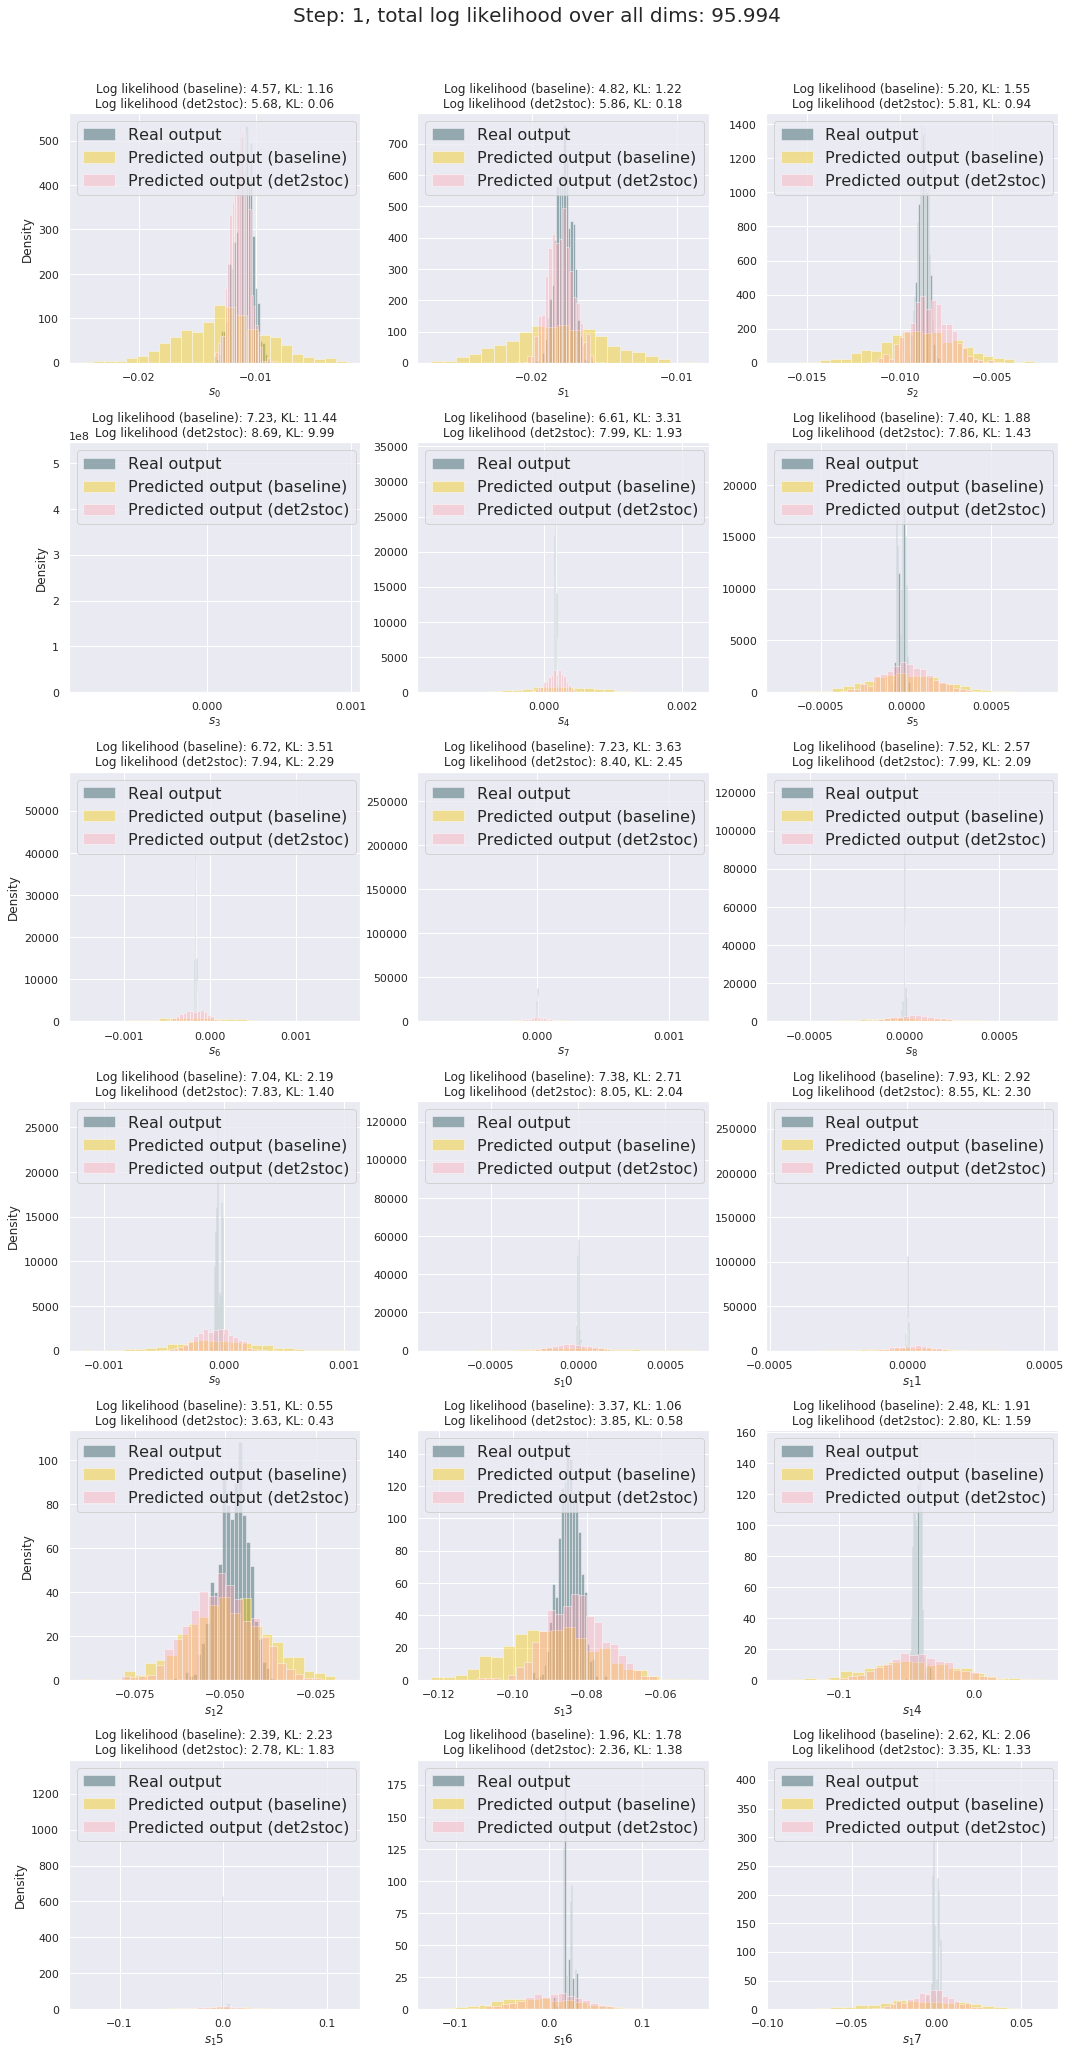
\includegraphics[trim=0 1650 0 50,clip,width=1.0\textwidth]
    {img/windyslope/output/output_distribution_step1_delta_all}
    \caption{$t=1$}
    \label{fig:output_distribution_step1_posvel_dettostoc}
\end{subfigure}
\begin{subfigure}{\textwidth}
    \centering
    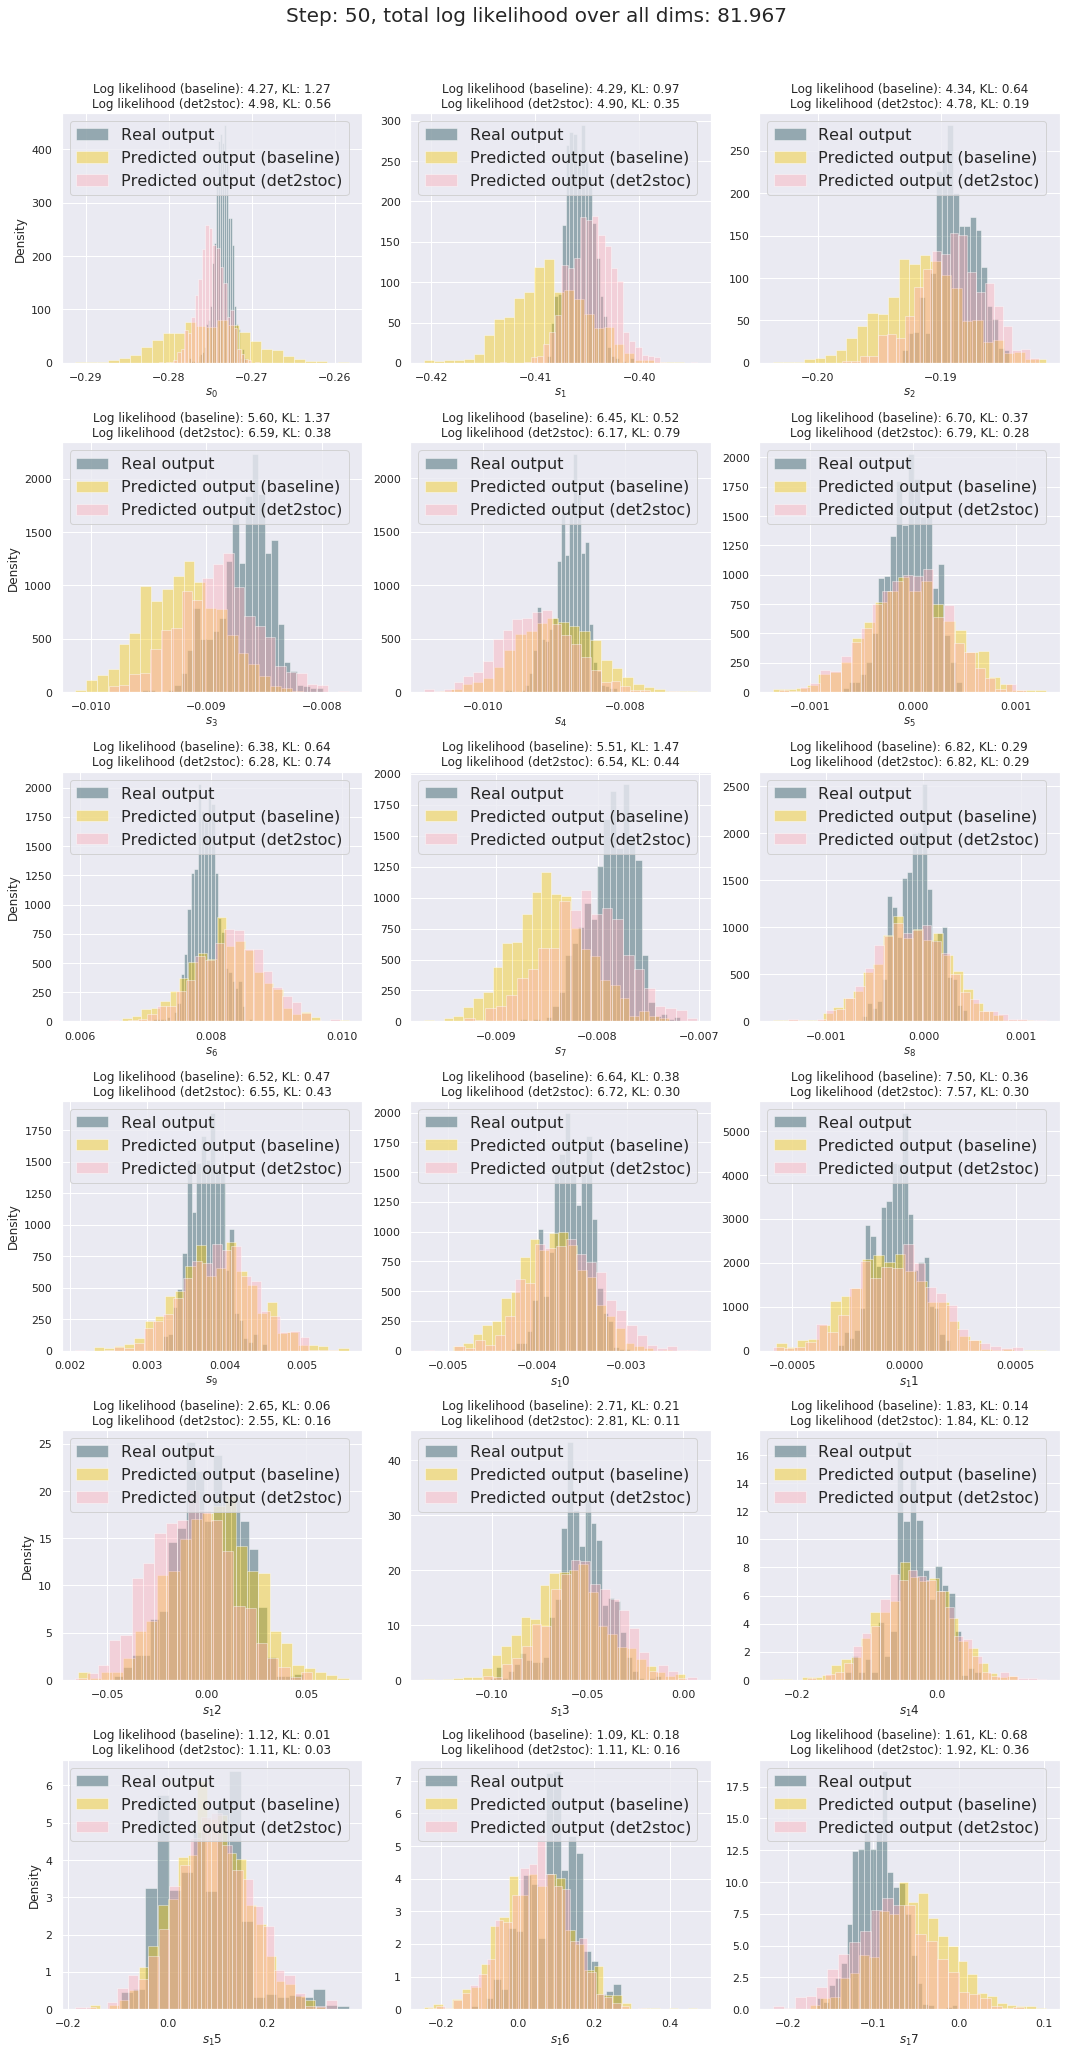
\includegraphics[trim=0 1650 0 50,clip,width=1.0\textwidth]
    {img/windyslope/output/output_distribution_step50_delta_all}
    \caption{$t=50$}
    \label{fig:output_distribution_step50_posvel_dettostoc}
\end{subfigure}
\begin{subfigure}{\textwidth}
    \centering
    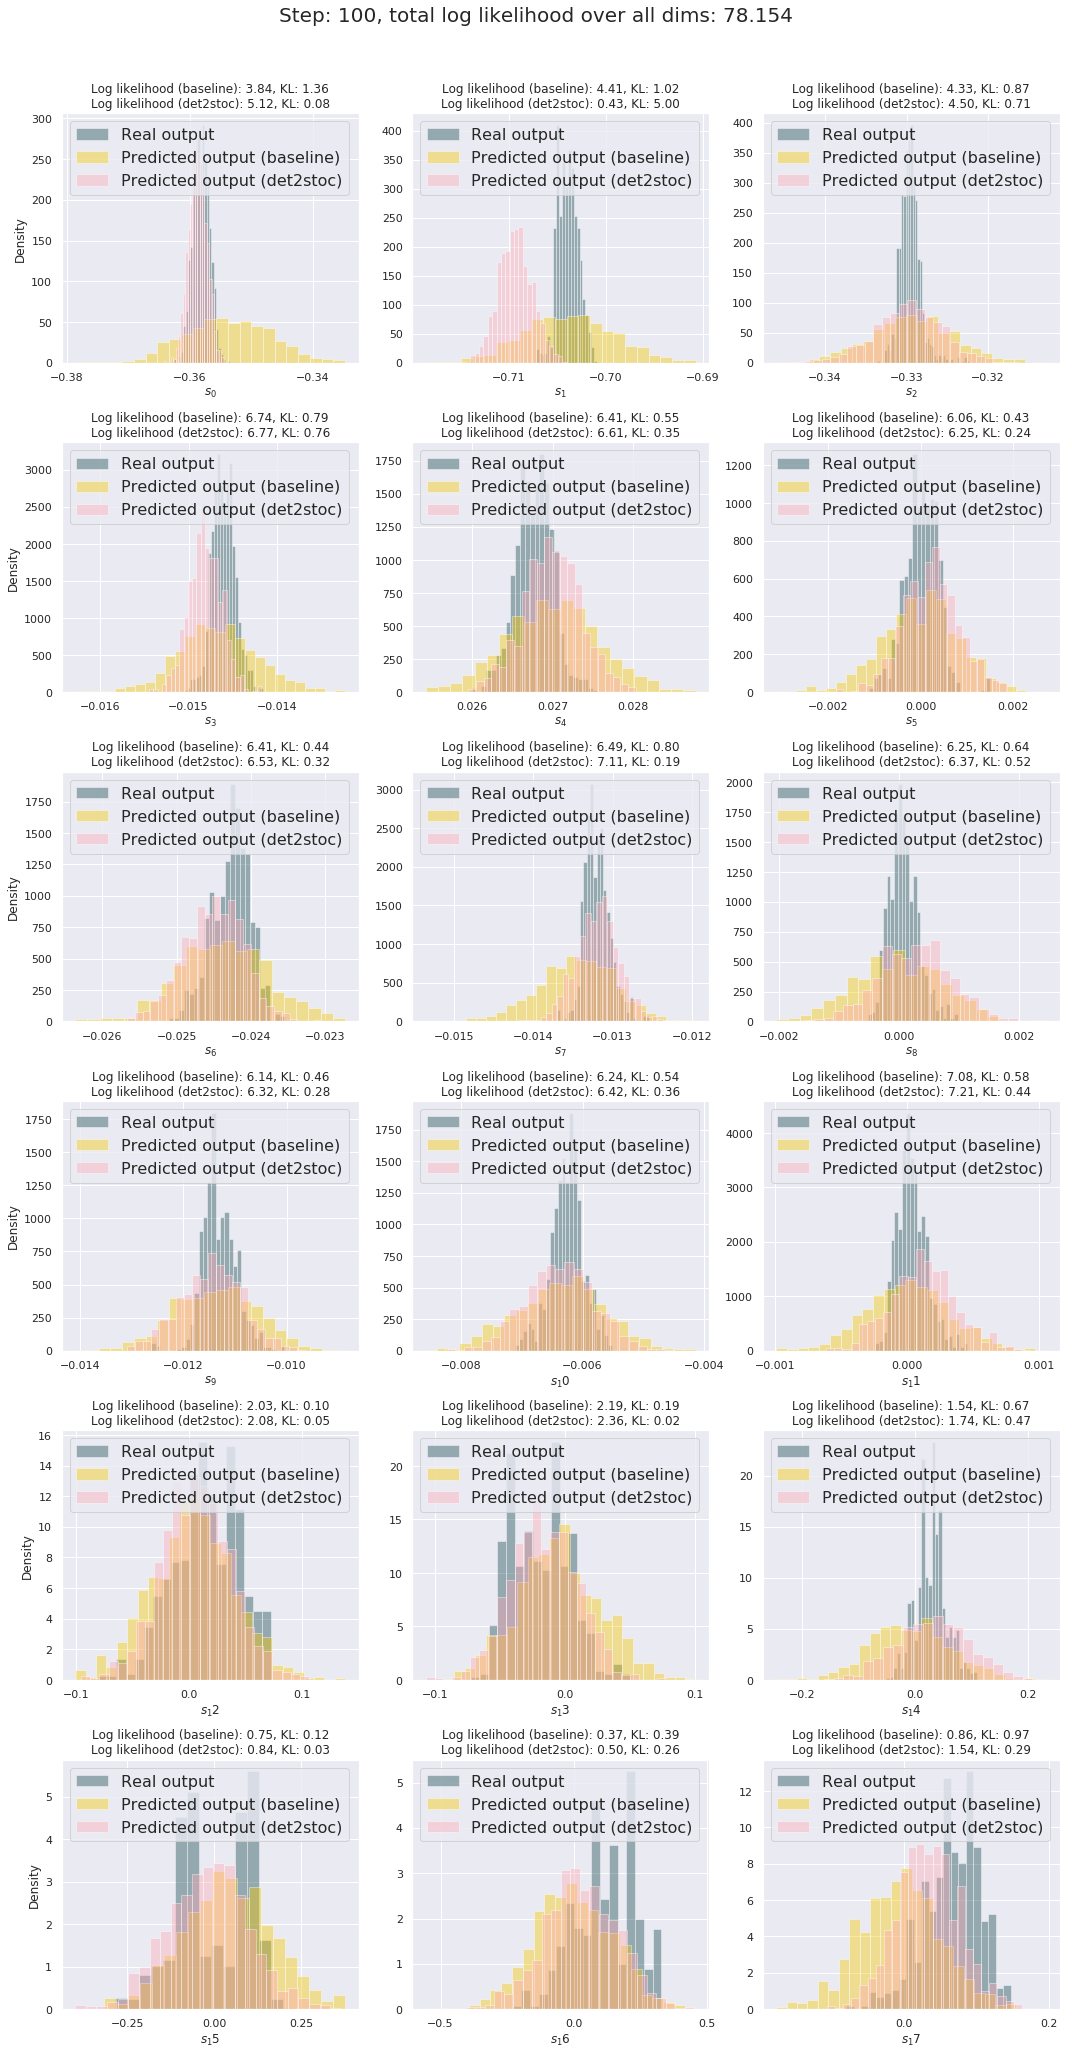
\includegraphics[trim=0 1650 0 50,clip,width=1.0\textwidth]
    {img/windyslope/output/output_distribution_step100_delta_all}
    \caption{$t=100$}
    \label{fig:output_distribution_step100_posvel_dettostoc}
\end{subfigure}
\caption{Prediction distributions $\ptheta \protect \given*{\vns}{\vs}$ for position outputs $(x,y,z)$ for a randomly sampled state at different timesteps $t$ for the simulator, the trained stochastic simulator trained with \dettostoc{} and the baseline. Above the plots are log likelihoods of the \emph{real} output as well as KL divergence between the predicted and true distributions per state dimension. The full state output can be found in Appendix \ref{appendix:a}.}
\end{figure}

The astute reader may wonder why we start with a lower number of \emph{real} trajectories which we incrementally increase in subsequent iterations of \dettostoc{}. When simulating passive dynamics, this does not make sense. However, in cases where we are trying to train an RL agent, we cannot explore all states of the environment in reasonable time by observing purely random actions. Instead, we propose to train a policy in simulation, perform rollouts in the real world, collect real observations and retrain the stochastic simulator with additional data. This is a process that can be repeated many times. For consistency, the data for this experiment was collected in a way that follows this principle.

\subsection{Retrieving parameter predictions using latent space codes}

As an experiment to see if \dettostoc{} can recover the \emph{real} parameters used by the simulator $\fsimulator_{\vth}$, we compute the expected mean and standard deviation of the posterior over the \emph{real} training set $\trajreal$. Since we have included the target $\vns$ in the posterior formulation, and pre-trained the decoder to match \fsimulator{}, samples from $\qphi \given{\vz}{\vs, \vns}$ should align with the true parameters $\vth$. The results can be seen in Table \ref{fig:windyslope_parameters_table} and visually in Figure \ref{fig:windyslope_latent_space}.
%$\E_{\given{\vz}{\vs, \vns}}$

\begin{table}[h!]
\ra{1.3}
\centering
\begin{tabular}{lrrcrr}
\multicolumn{6}{c}{\textsc{windy slope scenario}} \\
\toprule
%& \multicolumn{2}{c}{\small\emph{Real}} & \phantom{a} & \multicolumn{2}{c}{\emph{Sim}} \\
%\cmidrule{2-3} \cmidrule{5-6}
& $\theta_\mu^{(true)}$ & $\phi_\mu^{(learned)}$ && $\theta_\sigma^{(true)}$ & $\phi_\sigma^{(learned)}$ \\
\midrule
% $\N$(0.25, 0.1) 
% $\N$(0, 0.2)
% $\N$(-1, 1.0) 

$\pfriction$ & 0.23 & 0.2308 && 0.01 & 0.0105 \\
$\pcom$ & 0.11 & 0.1071 && 0.04 & 0.0520 \\
$\pwind$ & -1.7 & -1.7075 && 0.05 & 0.0546 \\
\bottomrule
\end{tabular}
\caption{Latent representations of parameters $\vpsi$ in the windy slope scenario after running three iterations of \dettostoc{} starting from fairly uninformative priors for the parameters $\vpsi$. $\theta_\mu$ and $\theta_\sigma$ correspond to the mean and standard deviation of the \emph{real} parameter distribution, and $\phi_\mu$ and $\phi_\sigma$ correspond to the mean and standard deviation of samples from the posterior over the collected \emph{real} trajectories $\trajreal$. The initial prior and posterior parameters after each iteration of \dettostoc{} can be found in Appendix \ref{appendix:a}.}
\label{fig:windyslope_parameters_table}
\end{table}

\begin{figure}[h!]
\centering
\captionsetup{size=footnotesize}
\begin{subfigure}{\linewidth}
  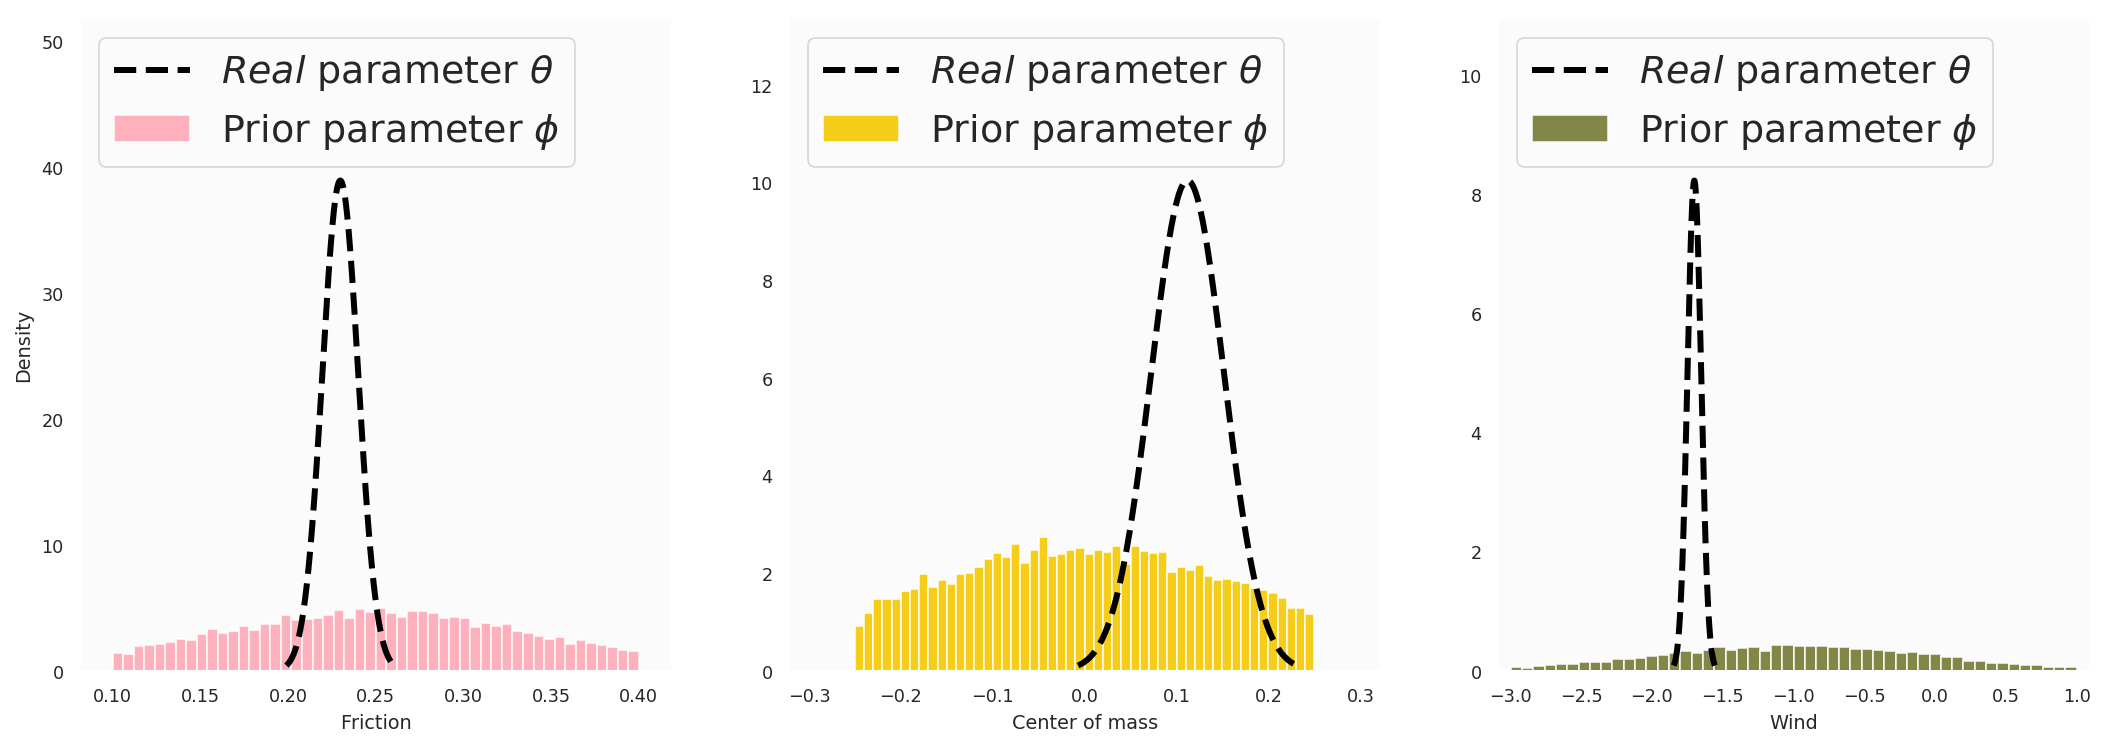
\includegraphics[width=1.0\linewidth]{img/windyslope/latent-representation/iter0_style_phi}
  \caption{Prior estimates}
\end{subfigure}
\begin{subfigure}{\textwidth}
  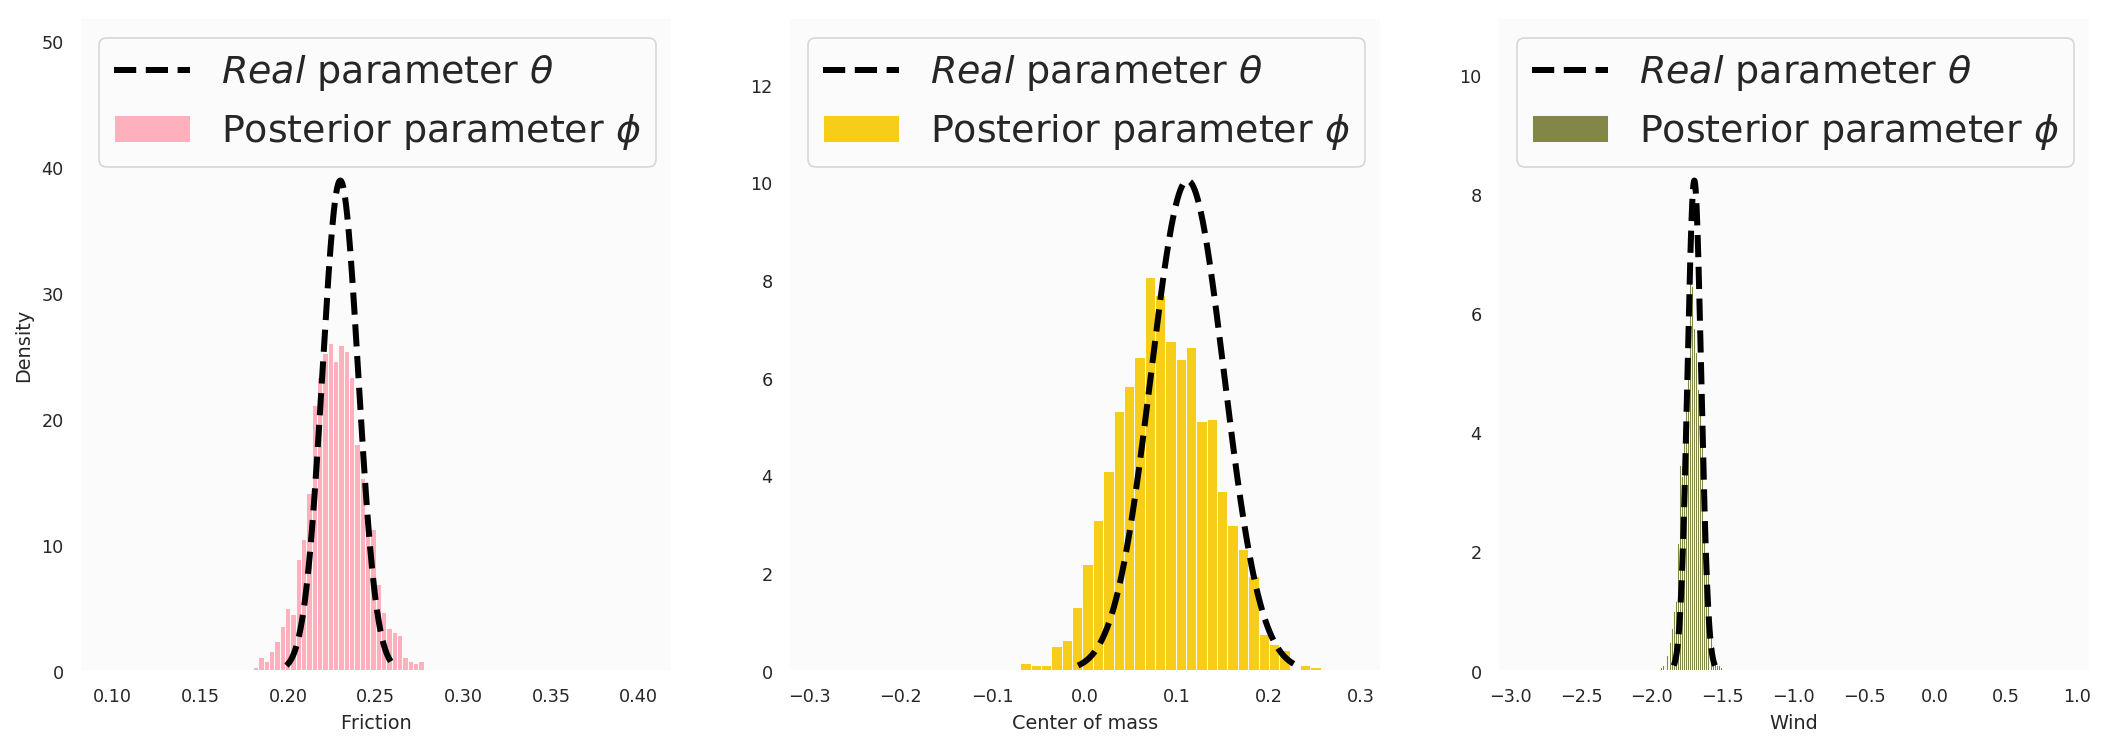
\includegraphics[width=1.0\linewidth]{img/windyslope/latent-representation/iter4_10_style}
  \caption{After 3 iterations of \dettostoc{}}
\end{subfigure}
\caption{Plots show the learned parameters $\vph_{\mu, \sigma}$ of the posterior given \emph{real} samples $\vec{\xi}^{real}$ as normalized histograms after 3 iterations of \dettostoc{}.
From left-to-right, the plots show tangential friction, center of mass and wind. The \emph{real} distribution of the parameters $\theta_{\mu, \sigma}$ in drawn with black dashes. Plots from previous iterations can be found in Figure \ref{fig:windyslope_latent_space_full} in Appendix \ref{appendix:a}.}
\label{fig:windyslope_latent_space}
\end{figure}

\clearpage
\section{\yp{} scenario}

A second scenario was constructed in MuJoCo that introduces control actions affecting the system dynamics. Similar to the Windy Slope scenario, a box with unknown center of mass is placed on a surface with unknown friction. However, inclination and wind have been removed and instead a robot interacts with the environment with the goal of pushing the box to a target goal.

The robot is an ABB IRB14000 YuMi with 2 arms, each with 7 joints corresponding to 14 degrees of freedom. The joints are actuated by velocity controllers. The real robot and the robot modelled in MuJoCo can be seen in Figure \ref{fig:robots}.

At the start of each episode, the arms are initialized to a default pose and the initial location of the box is placed randomly within a $0.2m \times 0.2m$ square area. The goal is kept fixed in the center of the table. The \emph{real} friction and center of mass distributions are listed in Table \ref{table:yumi_parameters}.

The goal is now to predict the next state $\vns$ given both $\vs$ and $\va$. The state consists of the position and velocity of all 14 joints, the position and orientations of the end effectors, as well as the position, rotation and velocity of the box.

The results can be found in Table \ref{table:yumi_results}. As the state vector is 60D we have chosen not to include the output distributions.

It should be noted that \dettostoc{} vastly outperforms the baseline even though it does overestimates the variance of $\pfriction{}$. This can be explained by the fact that the learned policy pushes the box in increments, and small changes in friction do not cause noticeable effects in the movement of the box. The posterior for all iterations can be found in Appendix \ref{appendix:a}.%In fact, we verified that replacing the learned posterior \pfriction{} with the true value $\theta_{friction}$ and this  

%The reward is a function of the distance: it is 0 outside a 0.14m radius of the goal, and otherwise monotonically increasing until the box is within 0.07m of the goal, which yields a reward of 1.


\begin{figure}%
    \centering
    \begin{subfigure}{0.4\textwidth}
    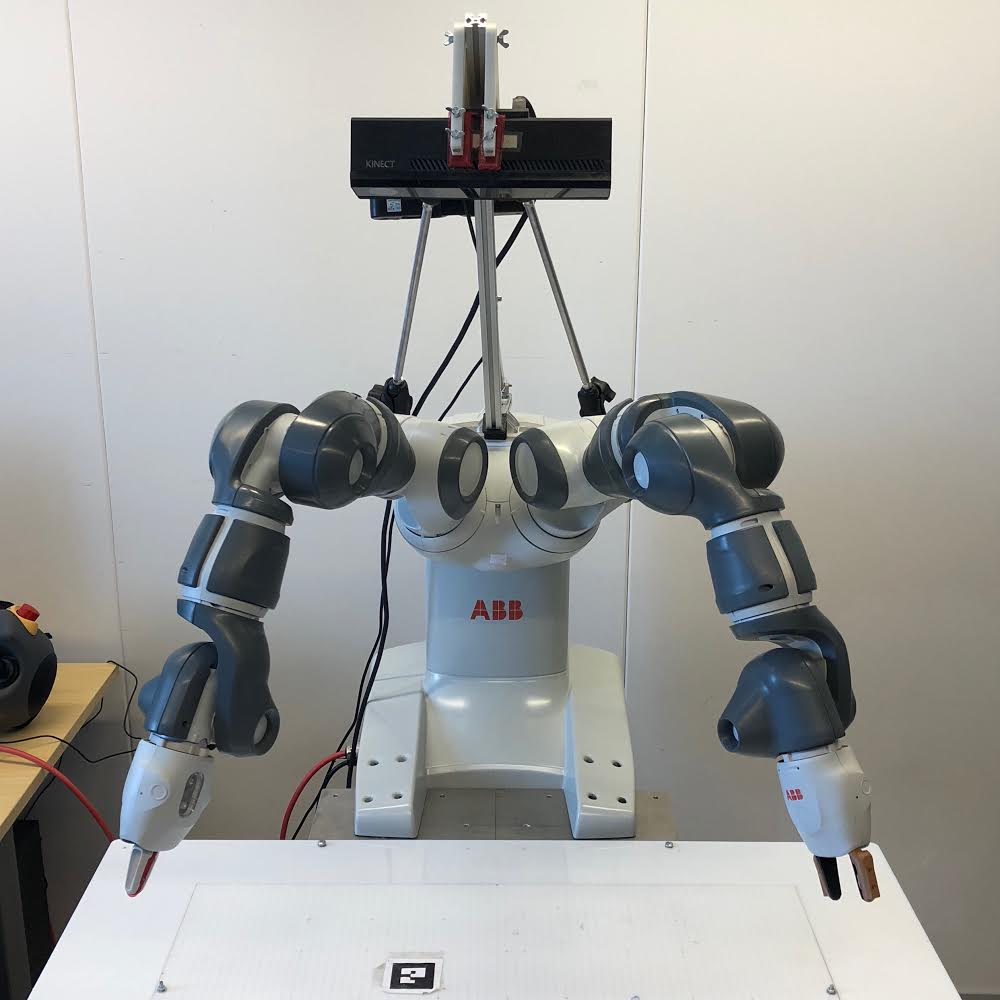
\includegraphics[width=1\textwidth,trim=0 0 0 0,clip]{img/yumi/yumi-pose-real}
    \end{subfigure}
    % \begin{subfigure}{0.4\textwidth}
    % 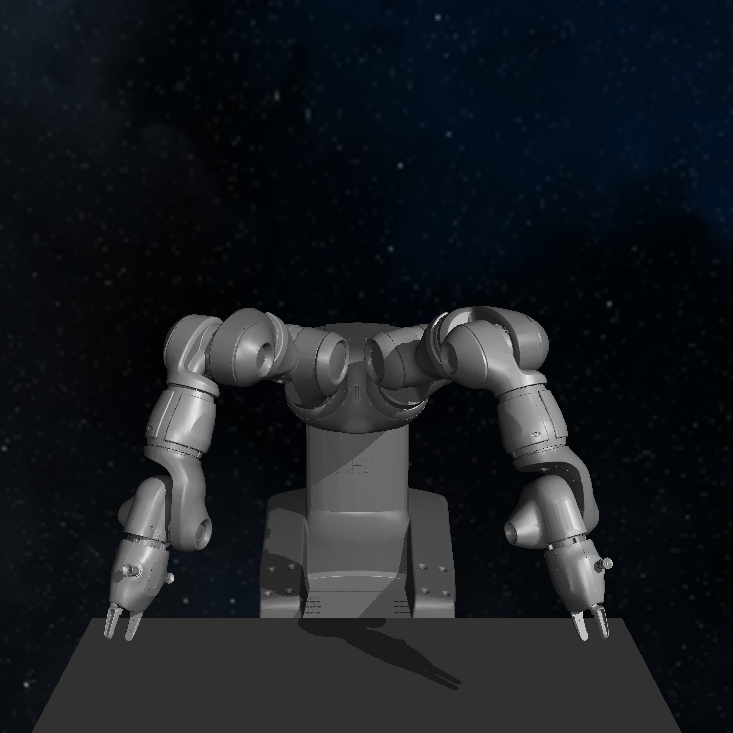
\includegraphics[width=1\textwidth]{img/yumi/yumi-pose-sim}
    % \end{subfigure}
    \begin{subfigure}{0.4\textwidth}
    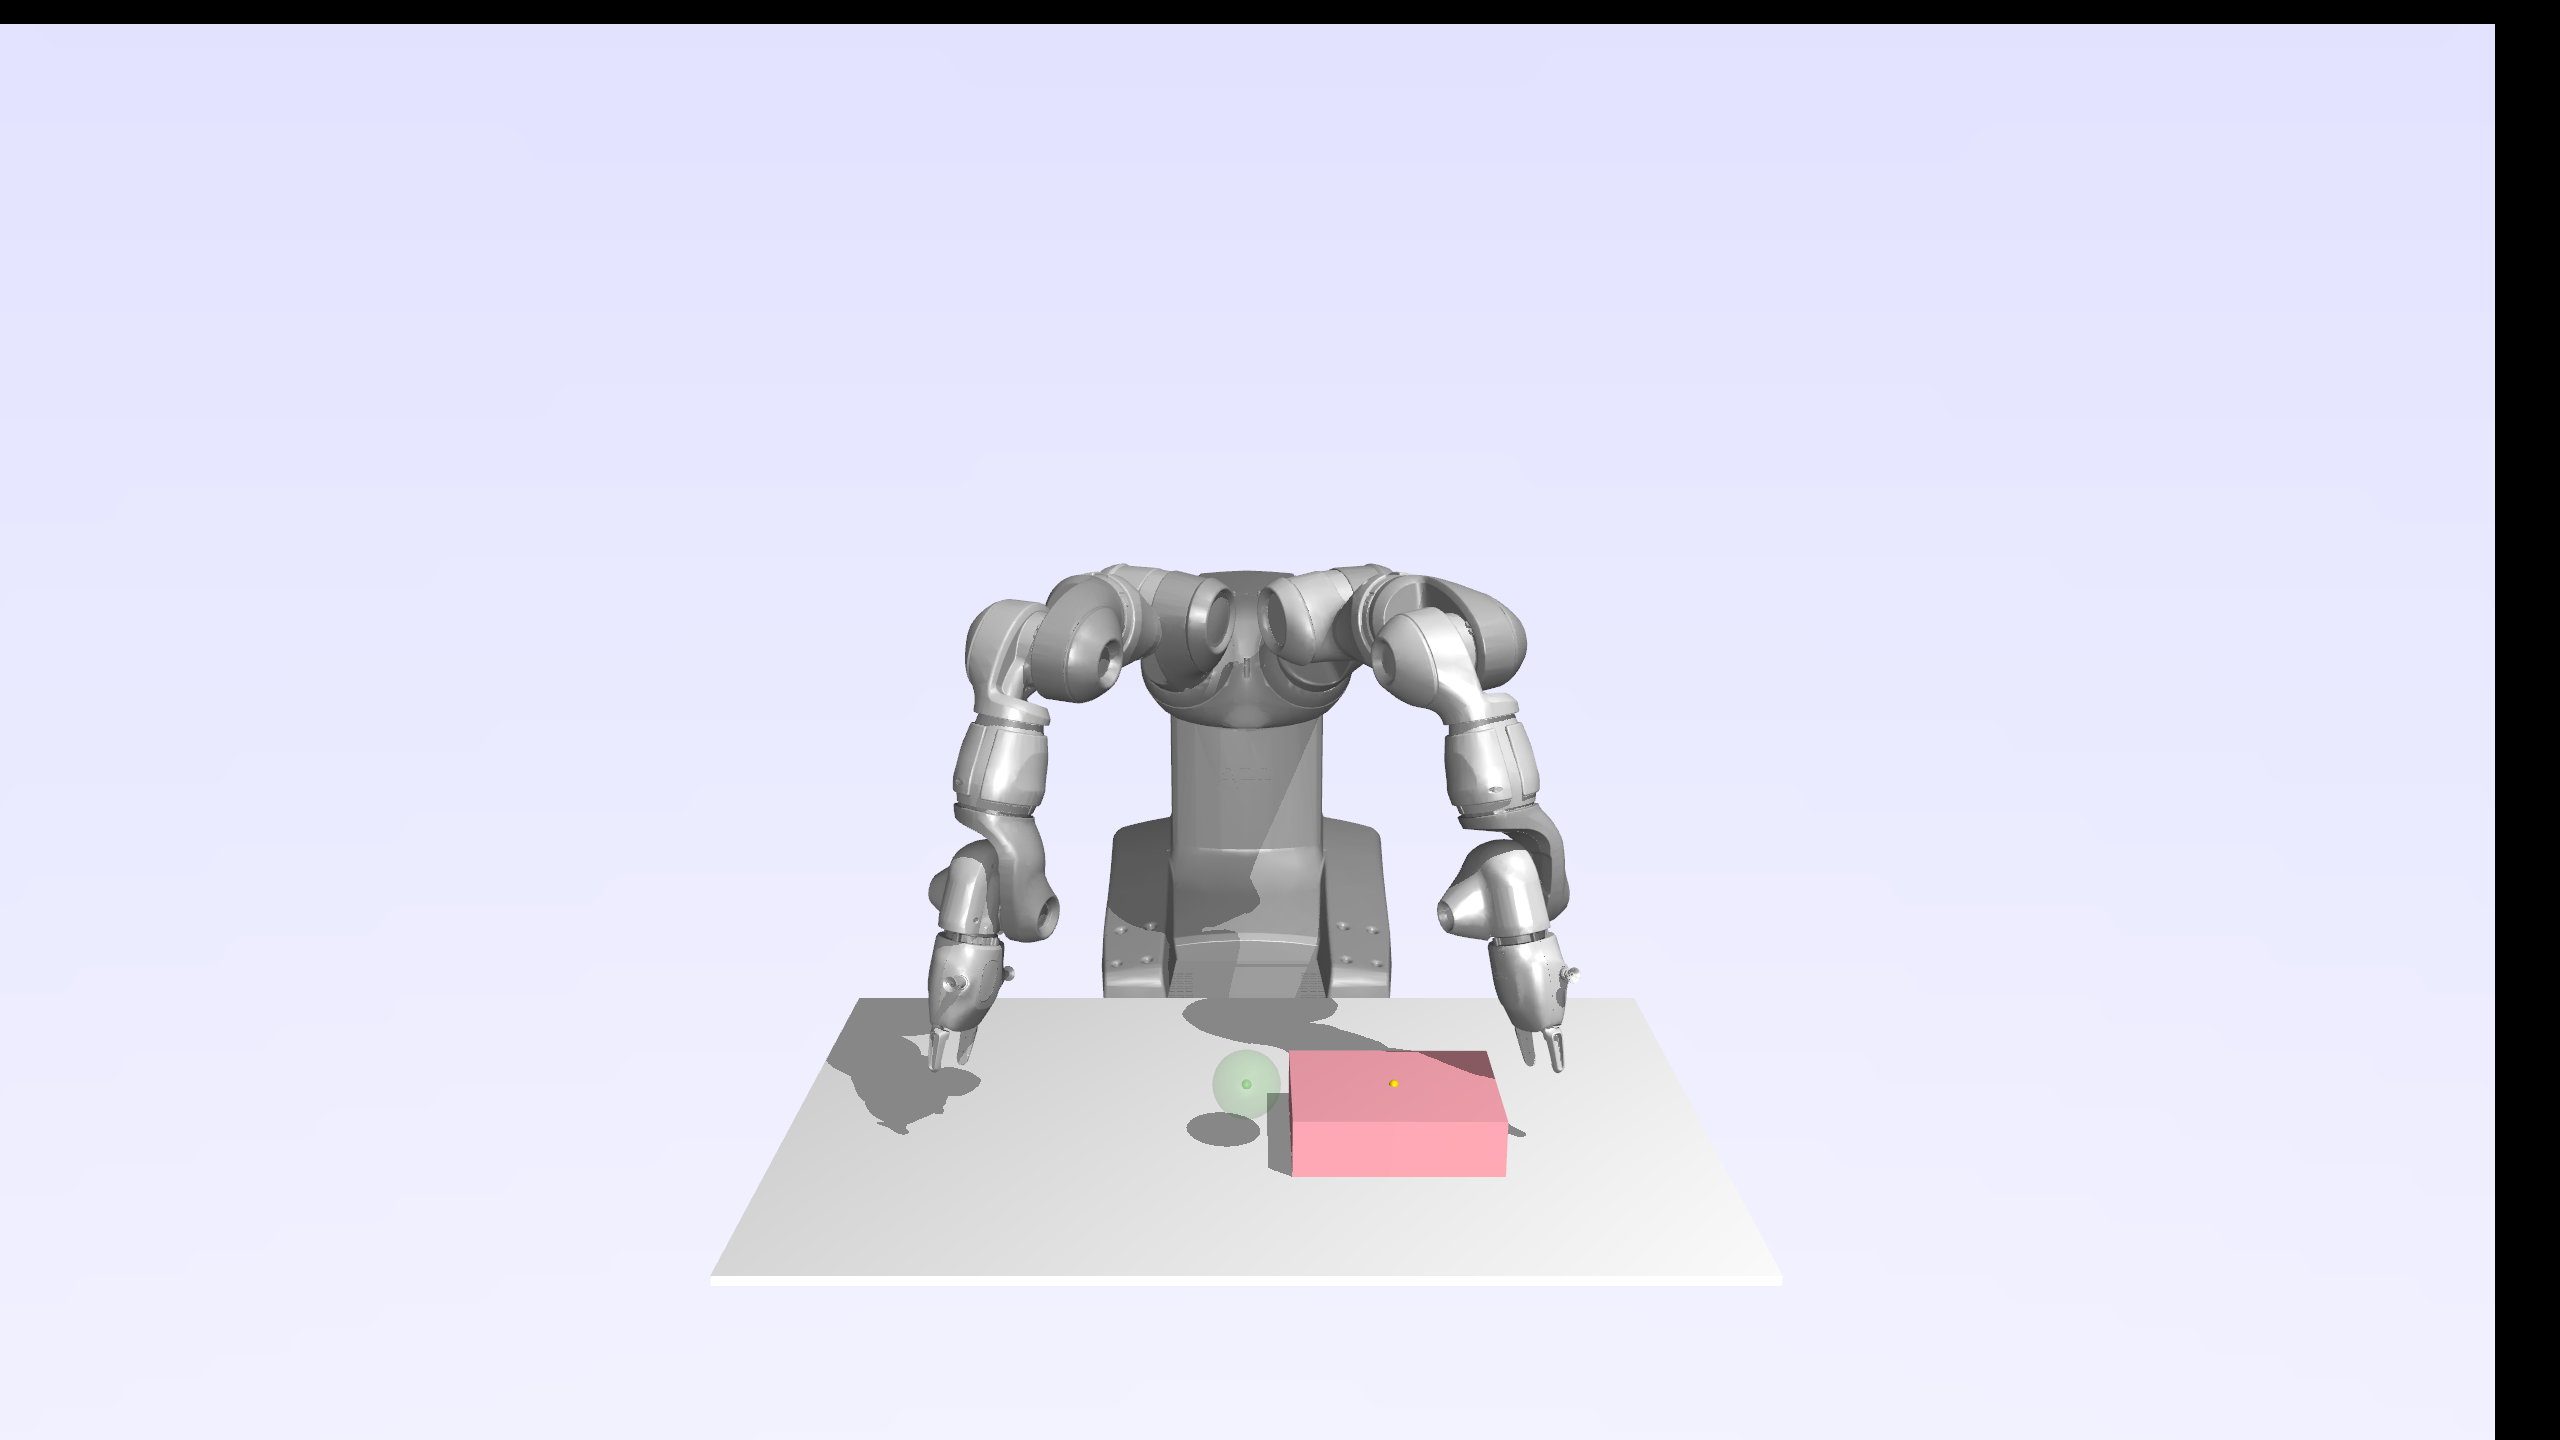
\includegraphics[width=1\textwidth,trim=800 240 810 250,clip]{img/yumi/yumi-pose-sim2}
    \end{subfigure}
    \caption{(Left) The real ABB YuMi IRB14000 robot. (Right) The robot modelled in MuJoCo for the \yp{} scenario. The environment is considered complete when the yellow sphere on the box is within the green sphere in the middle of the table.}
    \label{fig:robots}%
\end{figure}

\begin{table}
\ra{1.3}
\centering
\begin{tabular}{lrr}
\multicolumn{3}{c}{\textsc{\MakeLowercase{\yp{} scenario}}} \\
\toprule
%& \multicolumn{2}{c}{\small\emph{Real}} & \phantom{a} & \multicolumn{2}{c}{\emph{Sim}} \\
%\cmidrule{2-3} \cmidrule{5-6}
Model & \# \emph{Real} samples & Log likelihood of $\trajrealtest$ \\
\midrule
% 462.49237 463.926 488.15485 457.51343 481.58517 481.025
\cvae{} (baseline) & $1000$ & $472.45 \pm 11.54$\\
% 594.94806 615.2796 546.5111
%\cvae{} (baseline) & $10000$ & $585.58 \pm 25.27$ \\
% 648.6586 685.0386
\cvae{} (baseline) & $100000$ & $653.85 \pm 8.91$ \\
\dettostoc{} (1 iteration) & $600$ & $629.12 \pm 10.10$ \\
\dettostoc{} (2 iterations) & $800$ & $716.43 \pm 11.37$\\
\dettostoc{} (3 iterations) & $1000$ & \textbf{769.14 $\pm$ 12.32}\\

\bottomrule
\end{tabular}
\caption{Log likelihood results of the test set $\trajrealtest{}$ on the \yp{} scenario. \dettostoc{} has only seen 1000 \emph{real} samples (corresponding to 10 trajectories) but still outperforms the baseline model that has trained on 100000 samples.}
\label{table:yumi_results}
\end{table}

\begin{table}
\ra{1.3}
\centering
\begin{tabular}{lrrcrr}
\multicolumn{6}{c}{\textsc{\MakeLowercase{\yp{} scenario}}} \\
\toprule
%& \multicolumn{2}{c}{\small\emph{Real}} & \phantom{a} & \multicolumn{2}{c}{\emph{Sim}} \\
%\cmidrule{2-3} \cmidrule{5-6}
& $\theta_\mu^{(true)}$ & $\phi_\mu^{(learned)}$ && $\theta_\sigma^{(true)}$ & $\phi_\sigma^{(learned)}$ \\
\midrule
$\pfriction$ & $0.28$ & $0.2889$ && $0.01$ & $0.0431$ \\
$\pcom$ & $0.035$ & $ 0.0383$ && $0.005$ & $0.0056$ \\
\bottomrule
\end{tabular}
\caption{Latent representations of parameters $\psi$ in the \yp{} scenario after running two iterations of \dettostoc{} starting from uninformed priors for the parameters $\vec{\psi}$. $\theta_\mu$ and $\theta_\sigma$ correspond to the mean and standard deviation of the \emph{real} parameters of the distribution, and $\phi_\mu$ and $\phi_\sigma$ correspond to the mean and standard deviation of samples from the posterior over the collected \emph{real} trajectories $\vec{\xi}^{real}$.}
\label{table:yumi_parameters}
\end{table}

\begin{figure}
\centering
\captionsetup{size=footnotesize}
\begin{subfigure}{\textwidth}
  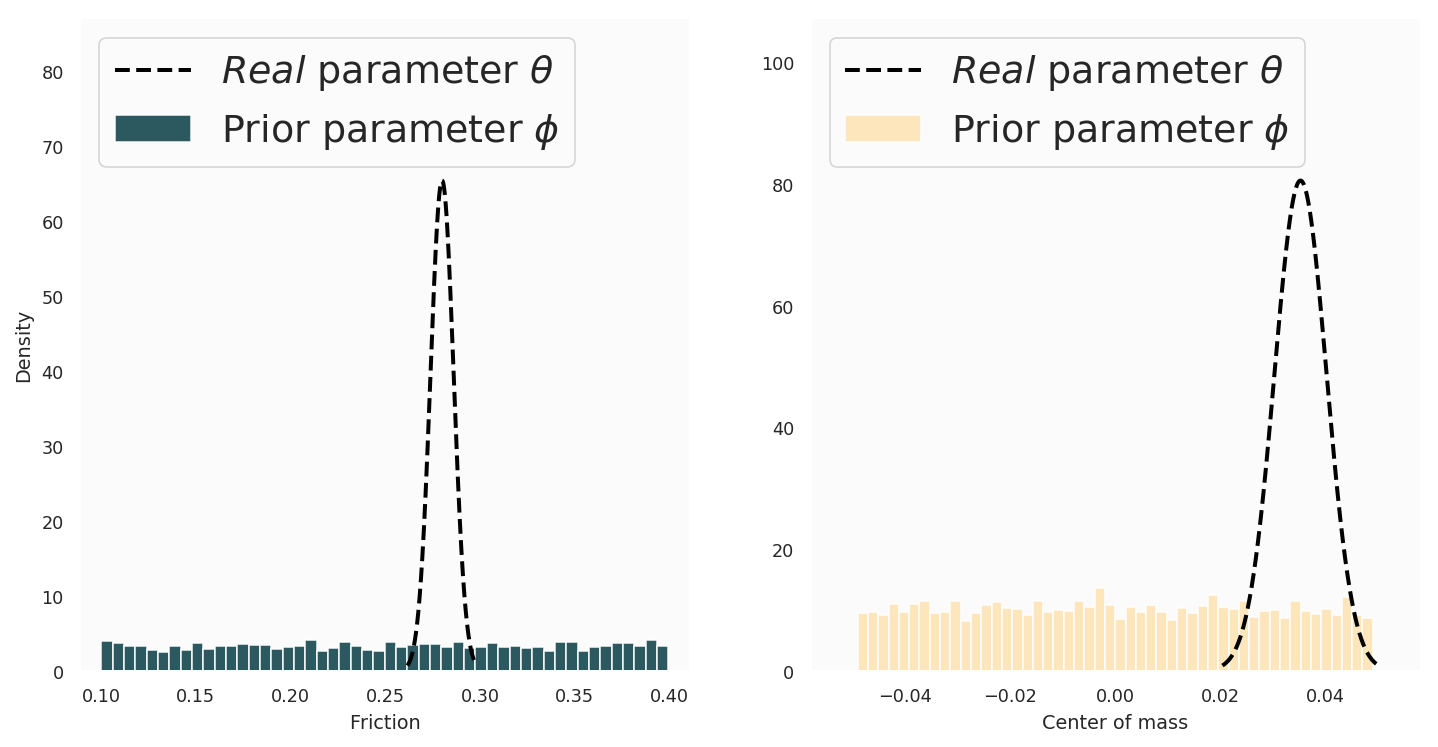
\includegraphics[width=\textwidth]{img/yumi/latent-representation/latent_encodings_iter0_style}%
  \caption{Prior estimates}
\end{subfigure}
\begin{subfigure}{\textwidth}
  \centering
  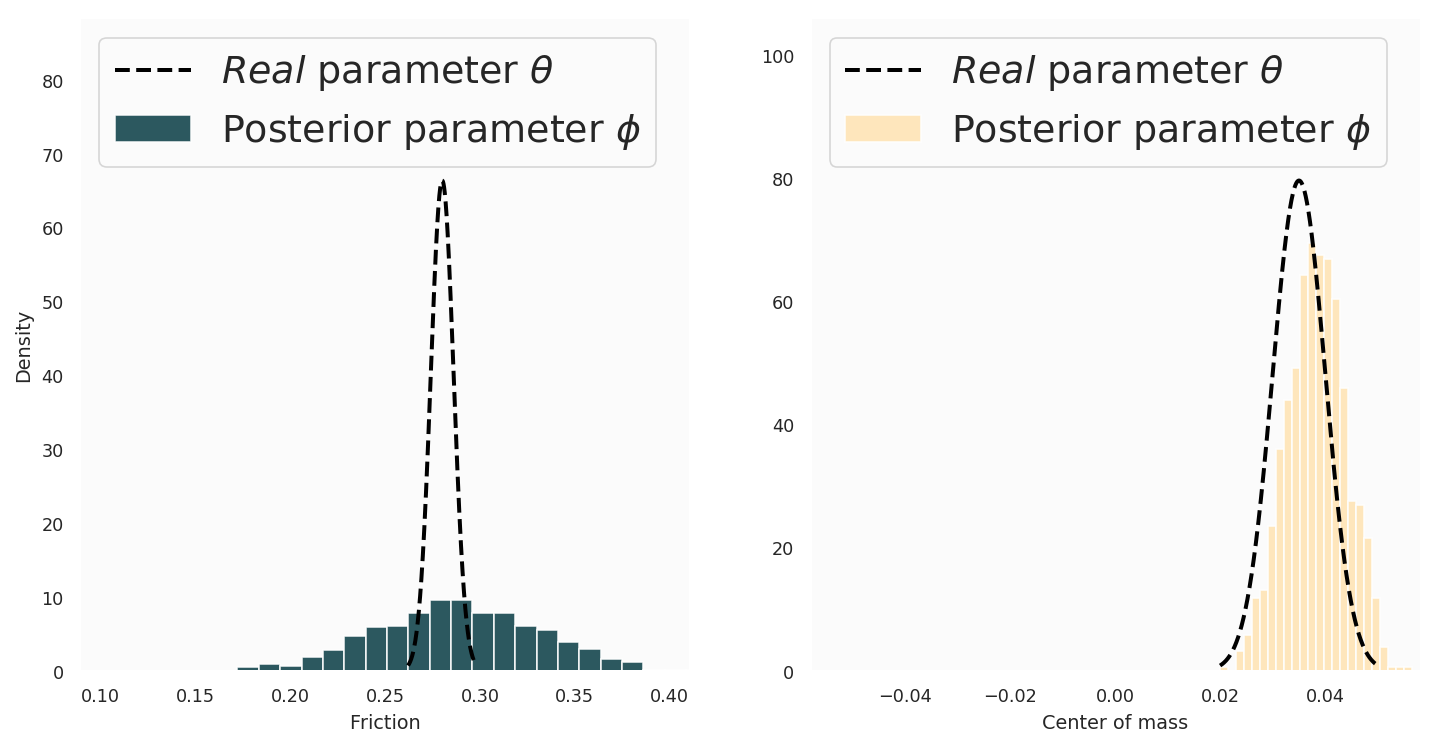
\includegraphics[width=\linewidth]{img/yumi/latent-representation/latent_encodings_iter4}
  \caption{After 3 iterations of \dettostoc{}}
\end{subfigure}
\caption{Plots show the prior parameters and learned parameters $\vph_{\mu, \sigma}$ of the posterior given \emph{real} samples $\trajreal{}$ for the \yp{} scenario after three iterations of \dettostoc{}. The parameters correspond (from left-to-right) to tangential friction $\pfriction$ and center of mass $\pcom$. The true distributions $\vth_{\mu, \sigma}$ are outlined in black dashes. In this scenario, \dettostoc{} struggles to match $\pfriction{}$ with the true distribution $\theta_\textsc{friction}$.}
\label{fig:yumi_latent_space}
\end{figure}

\section{Implementation details and Tools}

Since the KL divergence term in the objective function penalizes posteriors that diverge from the standard normal distribution, the simulator parameters are translated and scaled to have a mean of 0 and standard deviation of 1.

Rather than trying to output the next state, the target $\vy$ is the delta between next and current state $\vy_{\Delta} = \vns - \vs$.

The implementation of \dettostoc{} and the \ws{} scenario was written in Python 3.6, and the \yp{} scenario was written in C++. The neural networks were built using TensorFlow 1.13.1 \parencite{tensorflow2015-whitepaper}. We used MuJoCo Pro 1.50 as physics engine, including the Python wrapper by OpenAI.
%All experiments were conducted on a machine with a Intel Core i7-8700 CPU, NVIDIA GeForce 1080Ti and 16GB of RAM.